\section{Optimizations}\label{sec:optimizations}
The properties of the RVSDG make it an appealing IR for optimizing compilers. Many optimizations
can be expressed as simple graph traversals, where subgraphs are rewritten, nodes are moved between
regions, nodes or edges are marked, or edges are diverted. In this section, we present Common and
Dead Node Elimination optimizations that exploit the RVSDG's properties to unify traditionally
distinct transformations.

\subsection{Common Node Elimination}\label{sec:cne}
Common Node Elimination (CNE) permits the removal of redundant computations by detecting congruent
nodes. These nodes always produce the same results, enabling the redirection of their result edges
to a single node. This renders the other nodes dead, permitting Dead Node Elimination to remove
them. CNE is similar
to common subexpression elimination and value numbering~\cite{Alpern88} in that it detects
equivalent computations, but as the RVSDG represents all computations uniformly as nodes, it can
be extended to conditionals~\cite{Rugina00}, loops, and functions.

We consider two simple nodes $n_1$ and $n_2$ congruent, or $n_1 \cong n_2$, if they represent the
same computation, have the same number of inputs, \ie, $\card{I_{n_1}} = \card{I_{n_2}}$, and the
inputs $\iput{k}{n_1}$ and $\iput{k}{n_2}$ are congruent, or $\iput{k}{n_1} \cong \iput{k}{n_2}$,
for all $k = [0..\card{I_{n_1}}]$. Two inputs are congruent if their respective origins
$\origin{k}{n_1}$ and $\origin{k}{n_2}$ are congruent, \ie, $\origin{k}{n_1} \cong
\origin{k}{n_2}$. By definition, the origins of inputs are either outputs of simple or structural
nodes, or arguments of regions. Origins from simple nodes are only equivalent when their respective
producers are computationally equivalent, whereas for the other cases, it must be guaranteed that
they always receive the same value.

The implementation of CNE consists of two phases: mark and divert. The mark phase identifies
congruent simple nodes, while the divert phase diverts all edges of their origins to
a single node, rendering all other nodes dead. Both phases of Algorithm~\ref{alg:cne} perform a
simple top-down traversal, recursively processing subregions of structural nodes
annotating inputs, outputs, arguments, and results, as well as simple nodes as congruent. For
\gammanodes, the algorithm marks only computations within a \emph{single} region as congruent and
performs no analysis between regions. In the case of \thetanodes, computations are only congruent
when they are congruent before and after the loop execution, \ie, the inputs and results of two
loop variables must be congruent.
Figure~\ref{fig:dcne1} shows the RVSDG for the code in Figure~\ref{fig:dcne-code}, and Figure
\ref{fig:dcne2} the RVSDG after CNE. Two of the four multiplications take the same inputs and
therefore are congruent to each other, resulting in the redirection of their result edges.

\begin{informalg}{Common Node Elimination}{alg:cne}
\begin{enumerate}
	\vspace*{-0.7\baselineskip}

	\item \bpoint{Mark}: Process all nodes in topological order as follows:
		\begin{itemize}
			\item \bpoint{Simple nodes}: Denote this node as \n. Mark \n as congruent to all nodes
				\np which represent the same operation and where $\card{I_n} = \card{I_{n^{\prime}}} \land
				\iput{k}{n} \cong \iput{k}{n^{\prime}}$ for all $k = [0..\card{I_n}]$. Mark all outputs
				$\oput{k}{n} \cong \oput{k}{n^{\prime}}$ for all $k = [0..\card{O_n}]$.

			\item \bpoint{\gammanode}: For all entry variables $ev_1, ev_2 \in EV$ where
				$\iput{}{ev_1} \cong \iput{}{ev_2}$, mark $\argument{k}{ev_1} \cong \argument{k}{ev_2}$ for
				all $k \in [0..\card{A_{ev_1}}]$. Recursively process the \gammaregions. For all exit
				variables $ex_1, ex_2 \in EX$ where $\result{k}{ex_1} \cong \result{k}{ex_2}$ for all
				$k \in [0..\card{R_{ex_1}}]$, mark $\oput{}{ex_1} \cong \oput{}{ex_2}$.

			\item \bpoint{\thetanode}: For all loop variables $lv_1, lv_2 \in LV$ where
				$\iput{}{lv_1} \cong \iput{}{lv_2} \land \result{}{lv_1} \cong \result{}{lv_2}$, mark
				$\argument{}{lv_1} \cong \argument{}{lv_2}$ and $\oput{}{lv_1} \cong \oput{}{lv_2}$.
				Recursively process the \thetaregion.

			\item \bpoint{\lambdanode}: For all context variables $cv_1, cv_2 \in CV$ where
				$\iput{}{cv_1} \cong \iput{}{cv_2}$, mark $\argument{}{cv_1} \cong \argument{}{cv_2}$.
				Recursively process the \lambdaregion.

			\item \bpoint{\phinode}: For all context variables $cv_1, cv_2 \in CV$ where
				$\iput{}{cv_1} \cong \iput{}{cv_2}$, mark $a_{cv_1} \cong a_{cv_2}$. Recursively process
				the \phiregion.

			\item \bpoint{\omeganode}: Recursively process the \omegaregion.
		\end{itemize}

	\item \bpoint{Divert}: Process all nodes in topological order as follows:
		\begin{itemize}
			\item \bpoint{Simple nodes}: Denote this node as \n. For all nodes \np which are congruent to
				\n, divert all outputs $\oput{k}{n^{\prime}}$ to \oput{k}{n} for all $k = [0..\card{O_n}]$.

			\item \bpoint{\gammanode}: For all entry variables $ev_1, ev_2 \in EV$ where
				$\iput{}{ev_1} \cong \iput{}{ev_2}$, divert all edges from $\argument{k}{ev_2}$ to
				$\argument{k}{ev_1}$ for all $k \in [0..\card{A_{ev_1}}]$. Recursively
				process the \gammaregions. For all exit variables $ex_1, ex_2 \in EX$ where
				$\result{k}{ex_1} \cong \result{k}{ex_2}$ for all $k \in [0..\card{R_{ex_1}}]$, divert all
				edges from $\oput{}{ex_2}$ to $\oput{}{ex_1}$.

			\item \bpoint{\thetanode}: For all induction variables $lv_1, lv_2 \in LV$ where
				$\argument{}{lv_1} \cong \argument{}{lv_2} \land \oput{}{lv_1} \cong \oput{}{lv_2}$, divert
				all edges from $\argument{}{lv_2}$ to $\argument{}{lv_1}$ and from $\oput{}{lv_2}$ to
				$\oput{}{lv_1}$. Recursively process the \thetaregion.

			\item \bpoint{\lambdanode}: For all context variables $cv_1, cv_2 \in CV$ where
				$\iput{}{cv_1} \cong \iput{}{cv_2}$, divert all edges from $\argument{}{cv_2}$ to
				$\argument{}{cv_1}$. Recursively process the \lambdaregion.

			\item \bpoint{\phinode}: For all context variables $cv_1, cv_2 \in CV$ where
				$\iput{}{cv_1} \cong \iput{}{cv_2}$, divert all edges from $\argument{}{cv_2}$ to
				$\argument{}{cv_1}$. Recursively process the \phiregion.

			\item \bpoint{\omeganode}: Recursively process the \omegaregion.
		\end{itemize}

	\vspace*{-\baselineskip}
\end{enumerate}
\end{informalg}

For simple nodes, the algorithm marks all nodes within a
region that are congruent to a node \n. In order to avoid costly traversals of all nodes for every
node \n, the mark phase takes the candidates from the users of the origin of \n's first
input. If there is another input from a simple node \np with the same operation and number of
inputs among them, the other inputs from both nodes can be compared for congruence. Moreover, a
region must store constant nodes, \ie nodes without inputs, separately from other nodes so that the
candidate nodes for constants are available. For commutative simple nodes, the inputs should be
sorted before their comparison.

The presented algorithm only detects congruent simple nodes within a region. For \gammanodes,
congruence can also exist between nodes of different \gammaregions, and extending the
algorithm would eliminate these redundancies. Another extension would
be to detect congruent structural nodes, to implement conditional fusion
\cite{Rugina00} and loop fusion~\cite{manjikian97}. In
the case of \gammanodes, it is sufficient to ensure that two nodes have congruent
predicates, while \thetanodes require congruence detection between
different \thetaregions to ensure that their predicates are the same.



\subsection{Dead Node Elimination}\label{sec:dne}

\begin{figure*}
	\subfloat[Code\label{fig:dcne-code}]{
		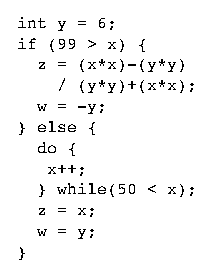
\includegraphics[scale=0.84]{code}
	}
	\hfill
	\subfloat[RVSDG\label{fig:dcne1}]{
		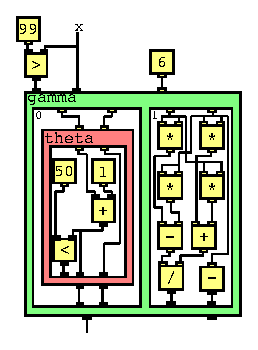
\includegraphics[scale=0.84]{dcne1}
	}
	\hfill
	\subfloat[After CNE\label{fig:dcne2}]{
		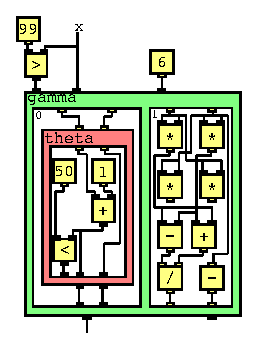
\includegraphics[scale=0.84]{dcne2}
	}
	\hfill
	\subfloat[After DNE mark\label{fig:dcne3}]{
		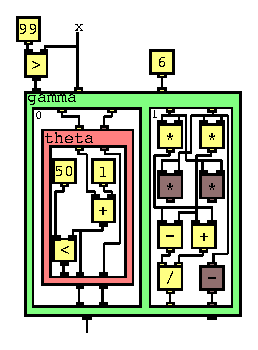
\includegraphics[scale=0.84]{dcne3}
	}
	\caption{Dead and Common Node Elimination}
	\label{fig:dcne}
\end{figure*}

Dead Node Elimination (DNE) is a combination of dead and unreachable code elimination, and removes
all nodes that do not contribute to the result of a computation. Dead nodes are generated by
unreachable and dead code from the input program, as well as by other
optimizations such as Common Node Elimination.
An operation is considered dead code when its results are either not used or only by
other dead operations. Thus, an output of a node is dead, if it has no users or all its users are
dead. We consider a node to be dead, if all its outputs are
dead. It follows that a node's inputs are dead, if the node itself is dead. We call all entities
that are not dead alive.

The implementation of DNE consists of two phases: mark and sweep. The mark phase identifies all
outputs and arguments that are alive, while the sweep phase removes all dead entities. The mark
phase traverses RVSDG edges according to the rules in Algorithm \ref{alg:dne}. If a structural
node is dead, the mark phase skips the traversal of its subregions as well as all of the contained
computations, as it never reaches the node in the first place. The mark phase is invoked for all
result origins of the \omegaregion.

The sweep phase performs a simple
bottom-up traversal of an RVSDG, recursively processing subregions of structural nodes as long as
these nodes are alive. A dead structural node is removed with all its contained computations.
The RVSDG's uniform representation of all computations as nodes permits DNE to not only remove
simple computations, but also compound computations such as conditionals, loops, or even entire
functions. Moreover, its nested structure avoids the processing of entire branches of the region
tree if they are dead.

\begin{informalg}{Dead Node Elimination}{alg:dne}
\begin{enumerate}
	\vspace*{-0.7\baselineskip}

	\item \bpoint{Mark}: Mark output or argument as alive and continue as follows:
		\begin{itemize}
			\item \bpoint{\omegaregion argument}: Stop marking.

			\item \bpoint{\phinode output}: Mark the result origin of the corresponding recursion
				variable.

			\item \bpoint{\phiregion argument}: Mark the input origin if the argument belongs to a
				context variable. Otherwise, mark the output of the corresponding recursion variable.

			\item \bpoint{\lambdanode output}: Mark all result origins of the \lambdaregion.

			\item \bpoint{\lambdaregion argument}: Mark the input origin if the argument is a dependency.

			\item \bpoint{\thetanode output}: Mark the \thetanode's predicate origin as well as the
				result and input origin of the corresponding loop variable.

			\item \bpoint{\thetaregion argument}: Mark the input origin and output of the corresponding
				loop variable.

			\item \bpoint{\gammanode output}: Mark the \gammanode's predicate origin as well as the
				origins of all results of the corresponding exit variable.

			\item \bpoint{\gammaregion argument}: Mark the input origin of the corresponding entry
				variable.

			\item \bpoint{Simple node output}: Mark the origin of all inputs.
		\end{itemize}

	\item \bpoint{Sweep}: Process all nodes in reverse topological order and remove them if they are
		dead. Otherwise, process them as follows:
		\begin{itemize}
			\item \bpoint{\omeganode}: Recursively process the \omegaregion. Remove all dead arguments.

			\item \bpoint{\gammanode}: For all exit variables $(R,o) \in EX$ where $o$ is dead, remove
				$o$ and all $r \in R$. Recursively process the \gammaregions. For all entry variables
				$(i,A) \in EV$ where all $a \in A$ are dead, remove all $a \in A$ and $i$.

			\item \bpoint{\thetanode}: For all loop variables $(i,a,r,o) \in LV$ where $a$ and $o$ are
				dead, remove $o$ and $r$. Recursively process the \thetaregion. Remove $i$ and $a$. 

			\item \bpoint{\lambdanode}: Recursively process the \lambdaregion. For all context variables
				$(i,a) \in CV$ where $a$ is dead, remove $a$ and $i$.

			\item \bpoint{\phinode}: For all recursion variables $(r, a, o) \in RV$ where $a$ and $o$ are
				dead, remove $o$ and $r$. Recursively process the \phiregion. Remove $a$. For all context
				variables $(i,a) \in CV$ where $a$ is dead, remove $a$ and $i$.
		\end{itemize}

	\vspace*{-\baselineskip}
\end{enumerate}
\end{informalg}

Figure~\ref{fig:dcne3} shows the RVSDG from Figure~\ref{fig:dcne2} after the mark phase.
Grey colored entities are dead. The mark phase traverses
the graph's edges, marking the \gammanode's leftmost output alive. This renders the
corresponding result origins of the \gammaregions alive, then the leftmost output of the
\thetanode, and so forth. After the mark phase annotated all outputs and arguments as alive, the
sweep phase removes all dead entities.


